\section{Анализ задания}
В рамках курса было необходимо разработать приложение, позволяющее продемонстрировать применение основных принципов проектирования программного обеспечения. В частности, в приложении необходимо было выделить следующие компоненты:

\begin{itemize}
\item Слой бизнес-логики
\item Слой хранения данных
\item Слой представления
\end{itemize}

Было решено разработать информационную систему для научного журнала.

\subsection{Роли}

В проекте выделено 3 роли: исследователь, редакция и рецензент:

\begin{itemize}
\item Исследователь

\begin{itemize}
\item Разрабатывает научную тему
\item Пишет статью по ней
\item Принимает замечания по ней
\item \textit{Цель:} Чтобы его статья была опубликована в журнале
\end{itemize}
\item Рецензент

\begin{itemize}
\item Выбирается редакцией
\item Получает статьи для просмотра
\item Дает оценку статье (стоит ли принимать для публикации)
\item Высказывает замечания, возникшие при прочтении статьи
\item \textit{Цель:} Выбрать подходящие статьи
\end{itemize}
\item Редакция

\begin{itemize}
\item Принимает статьи
\item Устанавливает правила принятия статей
\item Подбирает рецензентов
\item Связывает рецензентов и авторов
\item Корректирует статьи, если необходимо
\item Издает журнал с помощью типографии
\item \textit{Цель:} Принять качественные статьи, заработать на продаже журналов
\end{itemize}
\end{itemize}

\section{Варианты использования}

\subsection{Написание статьи}

\begin{enumerate}
\item
  \textbf{Исследователь} выбирает \textbf{тему} и при поддержке научного
  руководителя проводит исследования
\item
  По результататам исследований автор при поддержке соавторов пишет
  \textbf{научную статью}
\item
  Автор выбирает \textbf{журнал} для публикации
\item
  Автор получает от редакторов журнала \textbf{правила оформления}
\item
  Автор редактирует статью в соответствии с правилами
  
  \begin{itemize}
  \item
    Альтернатива: Редакция журнала сама готова привести
    \textbf{форматирование} к требуемому виду
  \end{itemize}
\end{enumerate}

\subsection{Подача}

\begin{enumerate}
\item
  Автор отправляет статью в \textbf{систему подачи статей}
\item
  \textbf{Редакция} просматривает статью
\item
  Статья передается на рецензирование
  
  \begin{itemize}
  \item
    Альтернатива: Редакция отказывает в приеме статьи и отправляет
    исследователю \textbf{список замечаний}, чтобы он их исправил
  \item
    Альтернатива: Редакция отказывает в приеме и рекомендует автору
    отправить статью в \textbf{другой журнал}
  \end{itemize}
\end{enumerate}

\subsection{Рецензирование}

\begin{enumerate}
\item
  Редакторы подбирают \textbf{рецензентов} и отправляют им статью
\item
  Рецензенты читают статью и составляют \textbf{отчет} по ней,
  содержащий \textbf{вопросы}, \textbf{замечания} и \textbf{общую оценку
  статьи}
\item
  Редакторы пересылают вопросы и замечания исследователю
\item
  В соответствии с оценкой редакция принимает \textbf{решение} о
  публикации
  
  \begin{itemize}
  \item
    Альтернатива: Редакция отказывает в публикации, статья дорабатывается
    и передается либо на этап рецензирования, либо на этап подачи, либо в
    другой журнал
  \end{itemize}
\end{enumerate}

\subsection{Подготовка и публикация}

\begin{enumerate}
\item
  Редакция адаптирует статью под \textbf{макет журнала}
\item
  Редакция исправляет \textbf{ошибки правописания}
\item
  Статья помещается в \textbf{пул публикаций}, которые будут
  опубликованы в следующем \textbf{выпуске} журнала
  \begin{itemize}
  \item
    Альтернатива: В дополнение к журналу, статья может быть
    \textbf{опубликована онлайн} индивидуально. Это происходит сразу же,
    без ожидания следующего выпуска журнала
  \end{itemize}
\item
  Журнал из статей отправляется в \textbf{типографию}
  \begin{itemize}
  \item
    Альтернатива: В дополнение к печатному варианту, журнал может быть
    опубликован в цифровом варианте
  \end{itemize}
\end{enumerate}

\subsection{Диаграмма вариантов использования}

\begin{figure}[H]
\centering
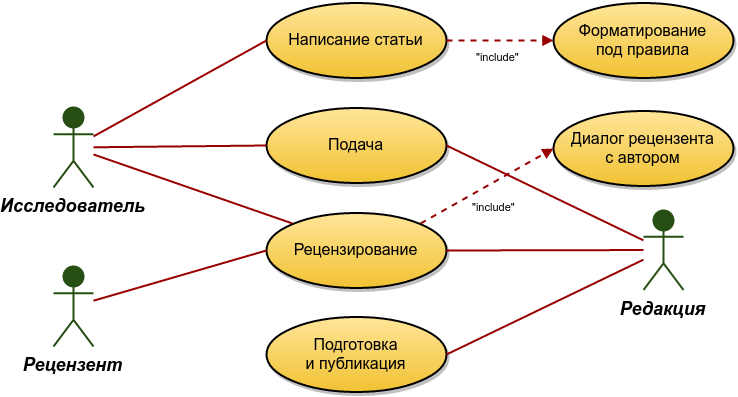
\includegraphics[width=\textwidth]{../UseCases.png}
\caption{Диаграмма вариантов использования}
\end{figure}

\subsection{Модель предметной области}

\begin{figure}[H]
\centering
\includegraphics[width=\textwidth]{../ClassDiagram.png}
\caption{Модель предметной области}
\end{figure}

\subsection{Диаграмма последовательностей}

\subsubsection{Написание статьи и отправка в
журнал}

\begin{figure}[H]
\centering
\includegraphics[width=\textwidth]{../Seq1.png}
\caption{}
\end{figure}

\subsubsection{Рецензирование}

\begin{figure}[H]
\centering
\includegraphics[width=\textwidth]{../Seq2.png}
\caption{}
\end{figure}

\section{Реализация задания с помощью технологии EJB}

\subsection{Объектно-ориентированное проектирование с учётом особенностей технологии}

Ниже приведена диаграмма классов для пакета objects, в котором содержатся классы, соответствующие сущностям предметной области. Альтернативы из вариантов использования представлены в приложении в виде перечислений Decision и Mark.

Для отслеживания состояния статьи используется перечисление State, имеющее варианты для каждого этапа обработки статьи.

\begin{figure}[H]
\centering
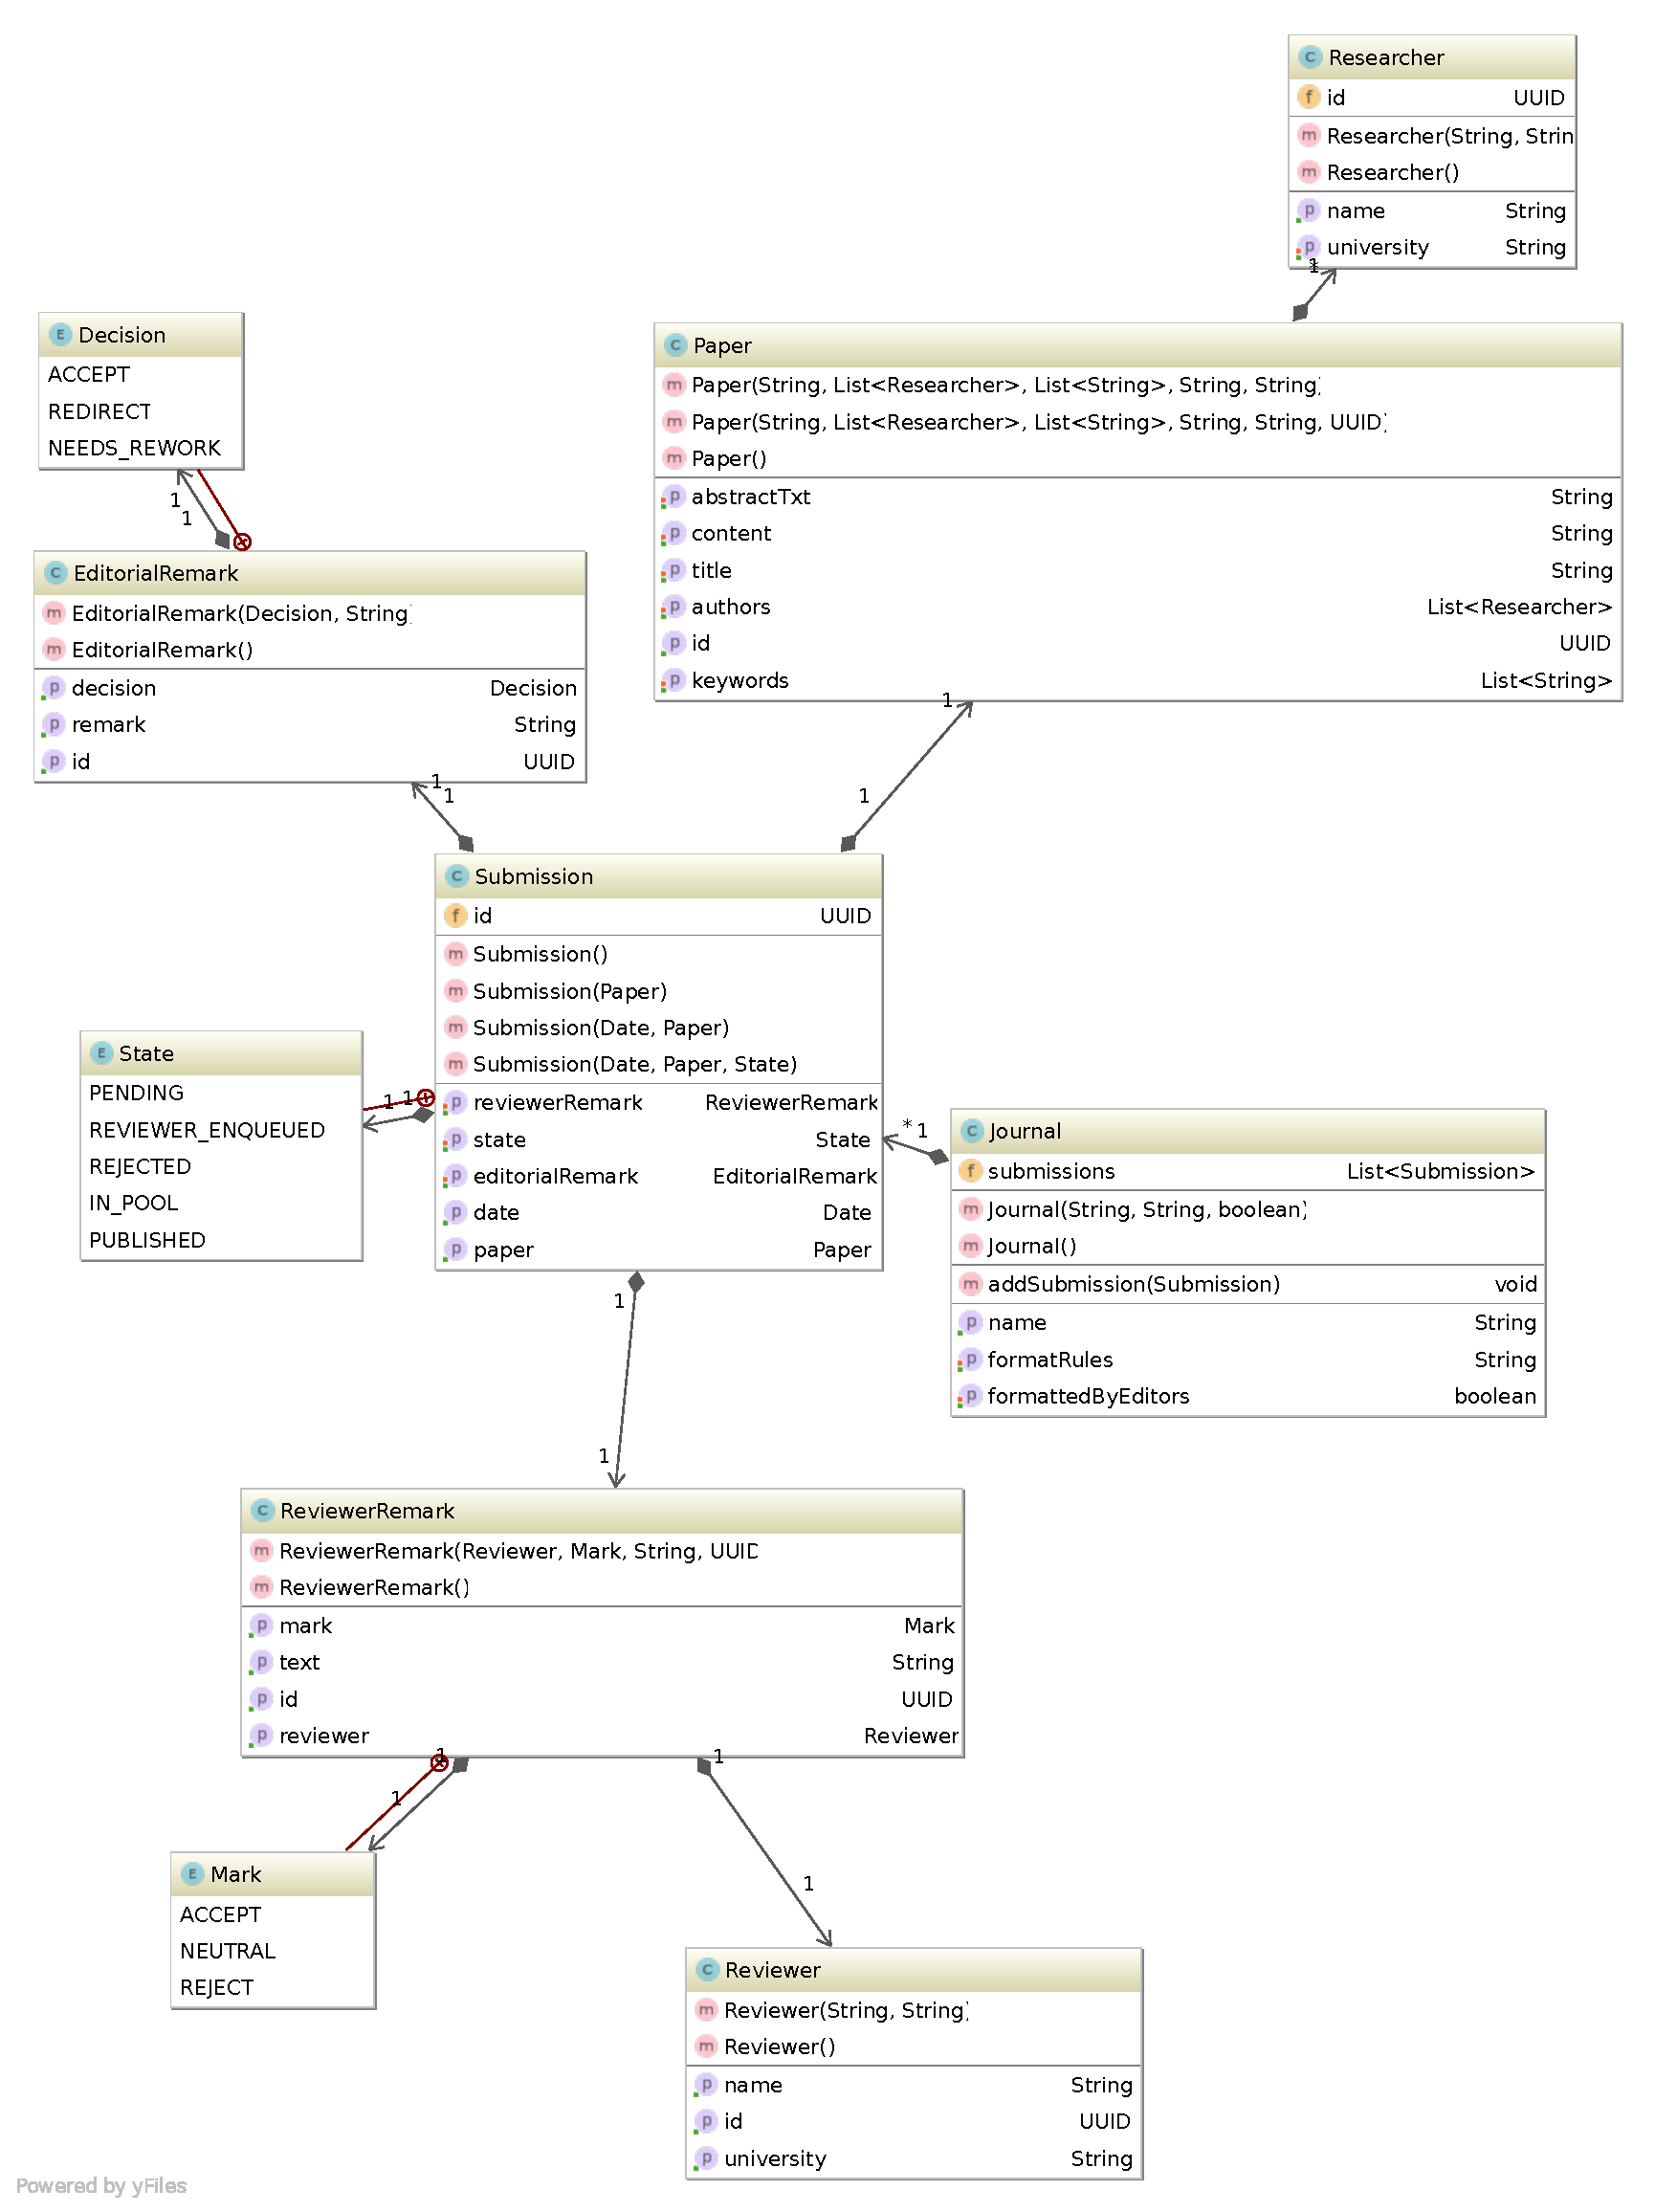
\includegraphics[width=\textwidth]{diagram.pdf}
\caption{Диаграмма класса для пакета objects}
\end{figure}

Ниже приведена диаграмма классов для пакетов services и repository, содержащих различные сервисы, используемые в приложении.

\begin{figure}[H]
\centering
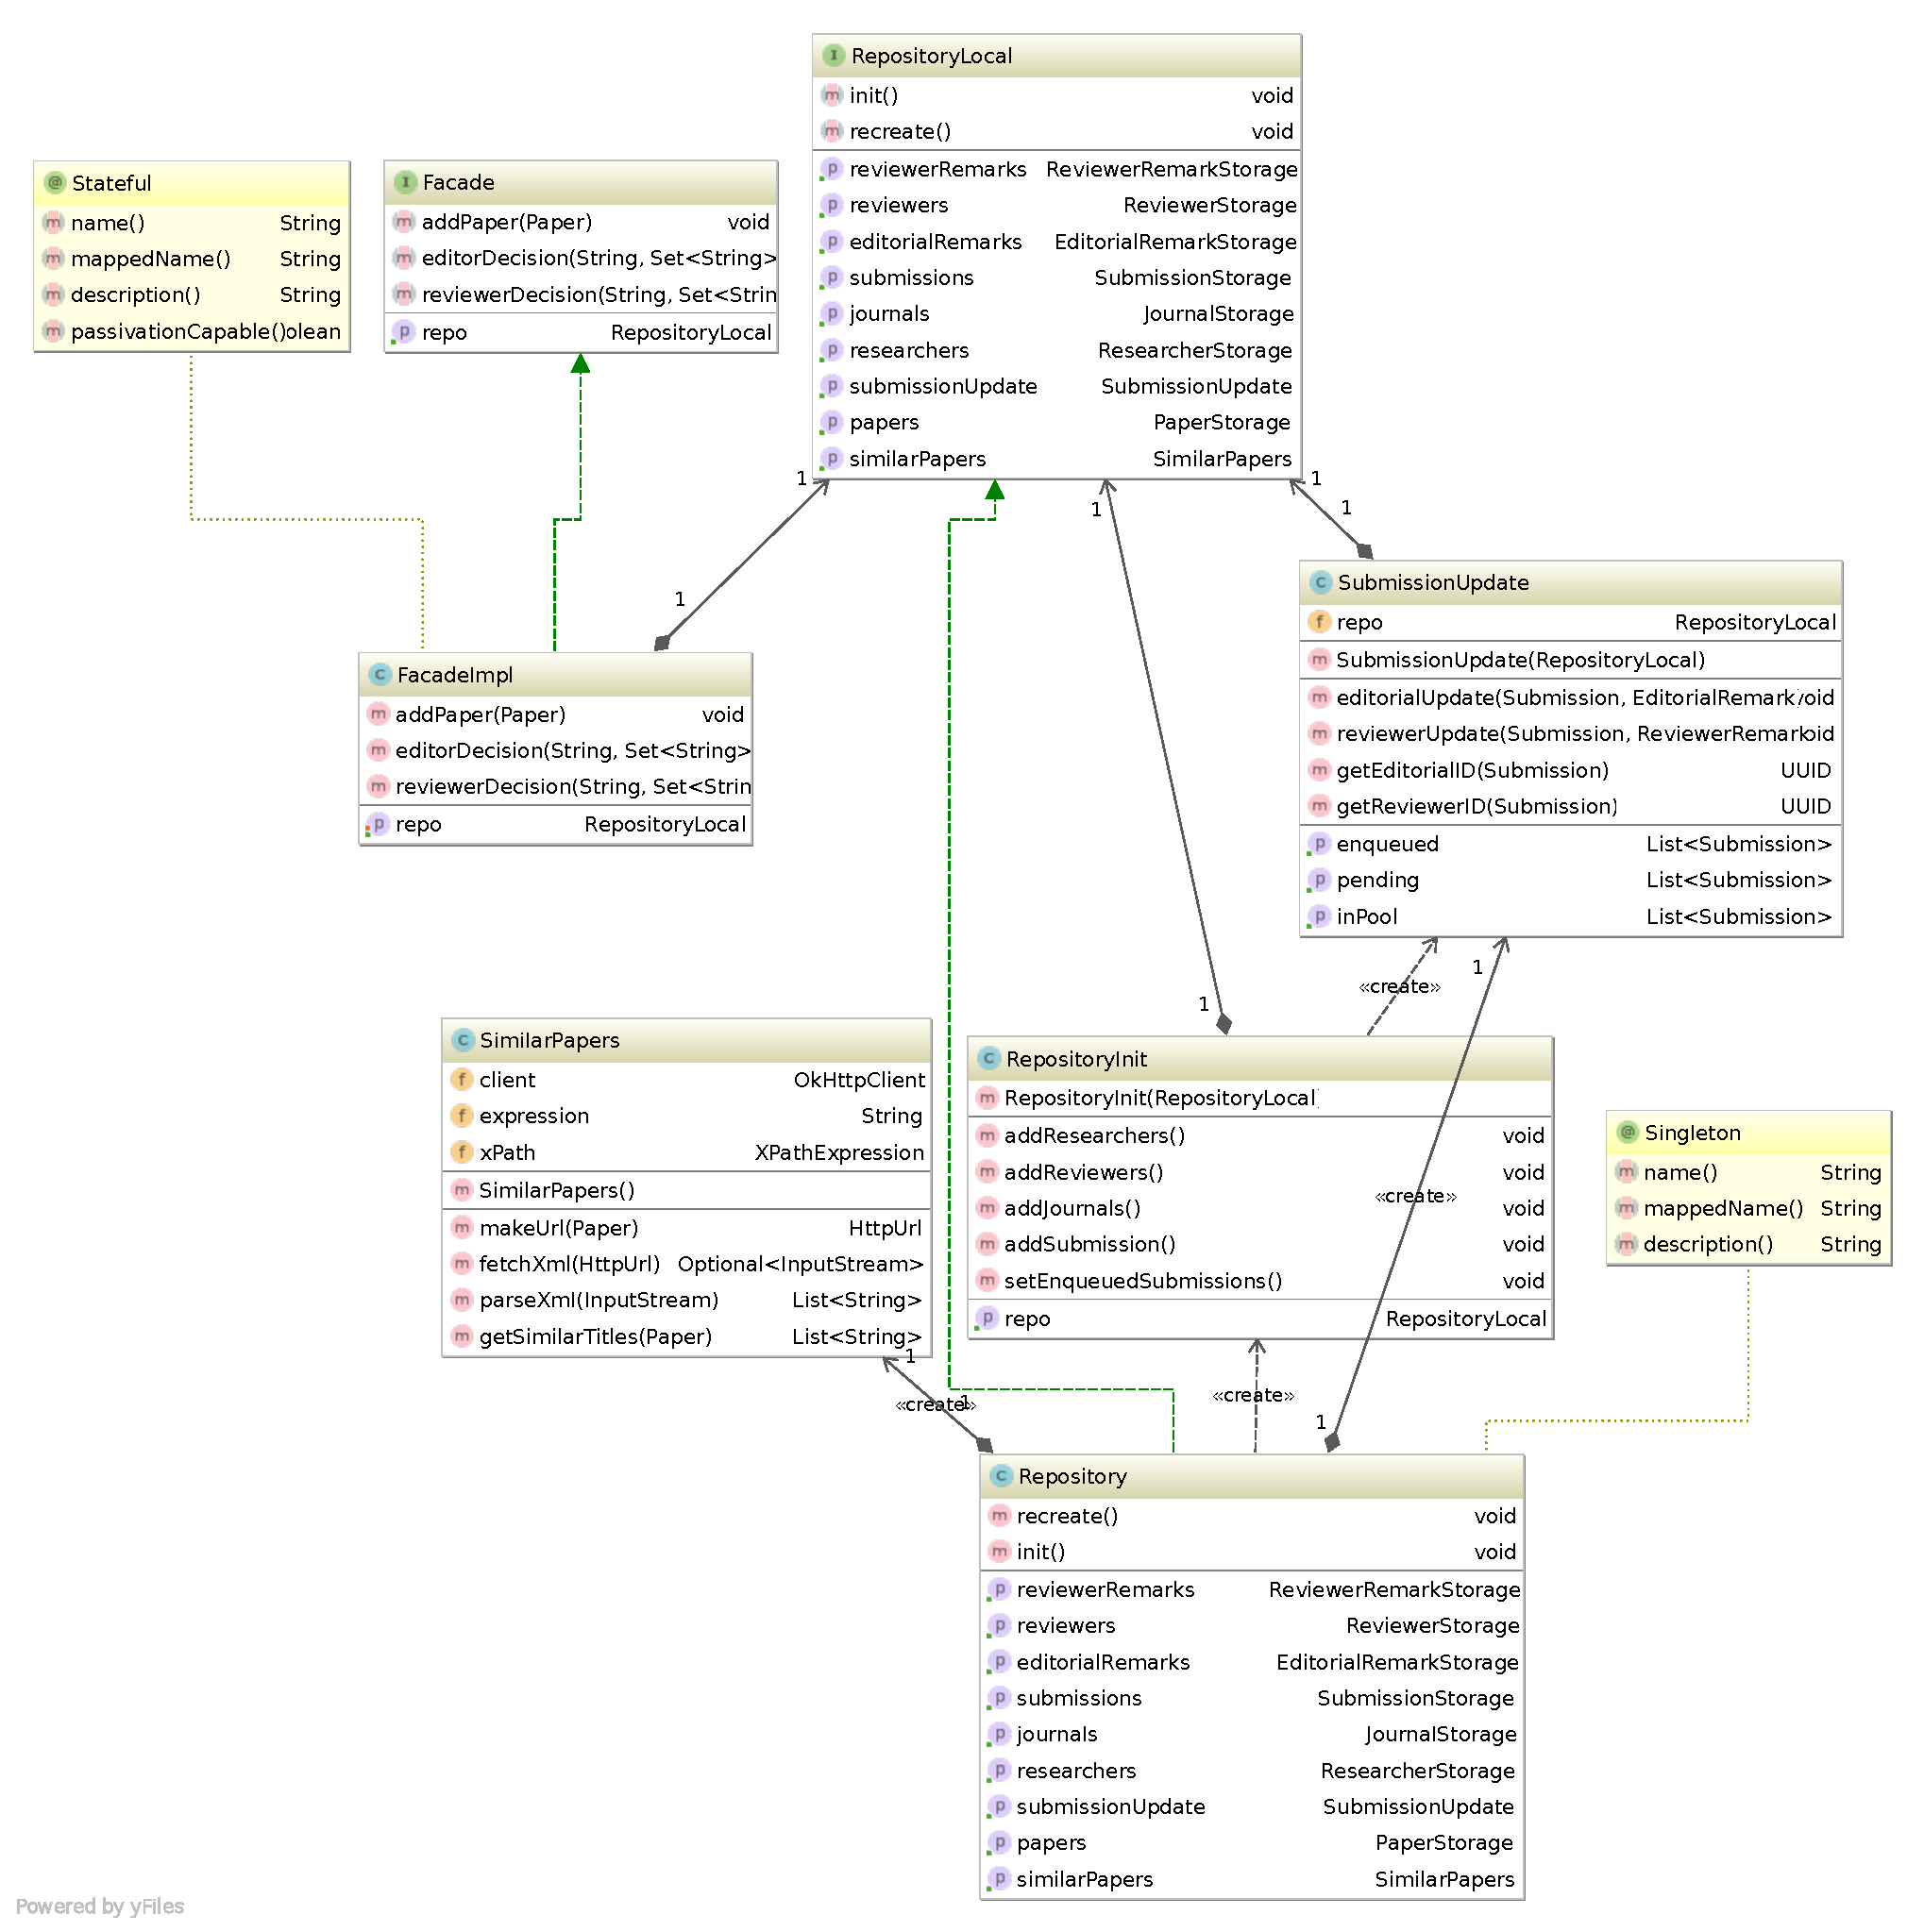
\includegraphics[width=\textwidth]{diagram2.pdf}
\caption{}
\end{figure}

На рисунке \ref{fig:mapper} показана диаграмма классов для слоя хранения.

\begin{figure}[H]
\centering
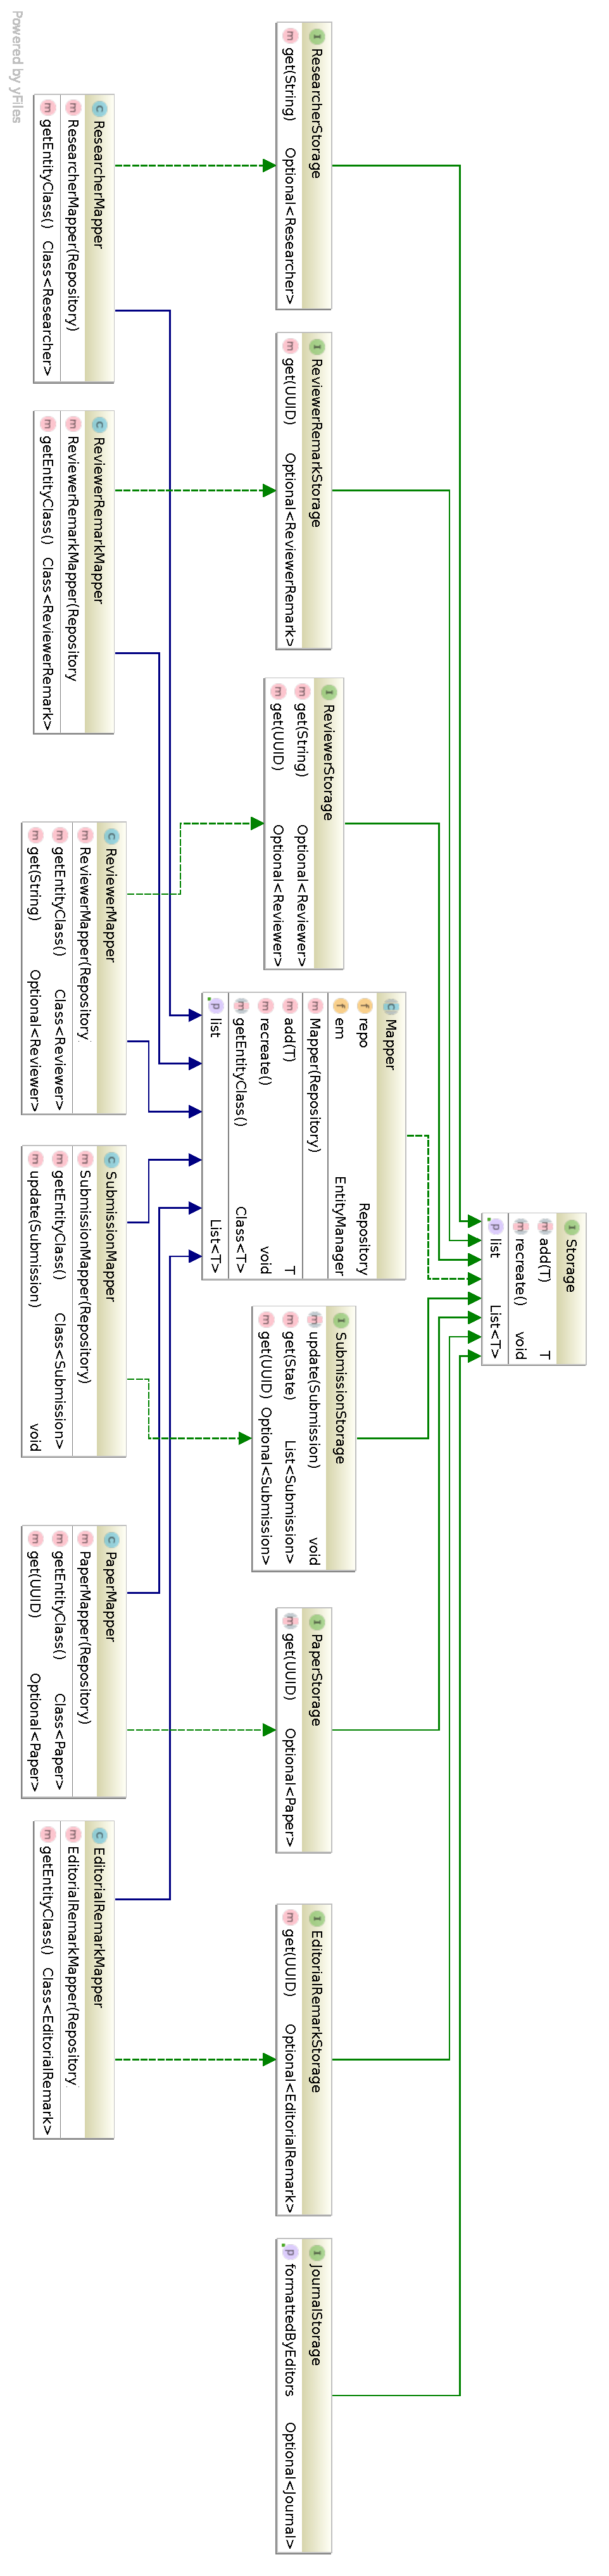
\includegraphics[height=0.97\textheight]{diagram3.pdf}
\caption{}
\label{fig:mapper}
\end{figure}

\subsection{Описание программы}

Было решено, что в приложении будет два bean-а:
\begin{enumerate}
\item Facade - класс для реализации паттерна проектирования <<Фасад>>. Соответствующий Bean было решено сделать @Stateful, чтобы исключить проблемы, связанные с одновременным использованием одного экземпляра класса несколькими клиентами.
\item Repository - класс-репозиторий, содержащий ссылки на объекты-Mapper-ы. Так как все клиенты используют общий набор Mapper-ов, класс Repository был помечен аннотацией @Singleton.
\end{enumerate}

Класс Facade содержит следующие методы:

\begin{itemize}
\item getRepo() - возвращает объект-репозиторий. Внутри класса Facade содержится поле repo, которое автоматически заполняется EJB-контейнером при создании нового экземпляра класса. Для этого поле repo было помечено аннотацией @EJB.
\item addPaper() - добавляет статью в базу данных, и создает для неё новый объект <<Подача>>.
\item editorDecision(String uuidString, Set<String> params, String remarkText) - для указанной статьи устанавливает решение редактора и добавляет примечание
\item reviewerDecision(String uuidString, Set<String> params, String user, String remarkText) - для указанной статьи устанавливает решение рецензента и добавляет примечание
\end{itemize}

\subsection{Инструкция системного администратора}

Для корректной работы проекта требуется установить следующее ПО:

\begin{itemize}
\item Пакет Java Runtime Environment 8
\item Сервер приложений WildFly 10
\end{itemize}

Для сборки проекта необходимо выполнить команду ./gradlew war:

\begin{lstlisting}
$ ./gradlew war
:clean
:compileJava
:processResources
:classes
:war

BUILD SUCCESSFUL

Total time: 0.946 secs
\end{lstlisting}

Собранный war-файл доступен по следующему пути: build/libs/\\SoftwareArchitecture.war

После сборки необходимо установить и настроить WildFly. С помощью скрипта add-user.sh добавим пользователя-администратора:

\begin{lstlisting}
artyom@artyom-MSI:~/Tools/wildfly-10.1.0.Final$ bin/add-user.sh 

What type of user do you wish to add? 
 a) Management User (mgmt-users.properties) 
 b) Application User (application-users.properties)
(a): 

Enter the details of the new user to add.
Using realm 'ManagementRealm' as discovered from the existing property files.
Username : user
Password recommendations are listed below. To modify these restrictions edit the add-user.properties configuration file.
 - The password should be different from the username
 - The password should not be one of the following restricted values {root, admin, administrator}
 - The password should contain at least 8 characters, 1 alphabetic character(s), 1 digit(s), 1 non-alphanumeric symbol(s)
Password : 
WFLYDM0099: Password should have at least 8 characters!
Are you sure you want to use the password entered yes/no? yes
Re-enter Password : 
What groups do you want this user to belong to? (Please enter a comma separated list, or leave blank for none)[  ]: 
About to add user 'user' for realm 'ManagementRealm'
Is this correct yes/no? yes
Added user 'user' to file '/home/artyom/Tools/wildfly-10.1.0.Final/standalone/configuration/mgmt-users.properties'
Added user 'user' to file '/home/artyom/Tools/wildfly-10.1.0.Final/domain/configuration/mgmt-users.properties'
Added user 'user' with groups  to file '/home/artyom/Tools/wildfly-10.1.0.Final/standalone/configuration/mgmt-groups.properties'
Added user 'user' with groups  to file '/home/artyom/Tools/wildfly-10.1.0.Final/domain/configuration/mgmt-groups.properties'
Is this new user going to be used for one AS process to connect to another AS process? 
e.g. for a slave host controller connecting to the master or for a Remoting connection for server to server EJB calls.
yes/no? no
\end{lstlisting}

После добавления пользователя можно запустить сам сервер приложений с помощью скрипта standalone.sh

\begin{lstlisting}
artyom@artyom-MSI:~/Tools/wildfly-10.1.0.Final$ bin/standalone.sh
=========================================================================

  JBoss Bootstrap Environment

  JBOSS_HOME: /home/artyom/Tools/wildfly-10.1.0.Final

  JAVA: /usr/lib/jvm/java-8-oracle/bin/java

  JAVA_OPTS:  -server -Xms64m -Xmx512m -XX:MetaspaceSize=96M -XX:MaxMetaspaceSize=256m -Djava.net.preferIPv4Stack=true -Djboss.modules.system.pkgs=org.jboss.byteman -Djava.awt.headless=true

=========================================================================
...
13:13:05,239 INFO  [org.jboss.as] (Controller Boot Thread) WFLYSRV0060: Http management interface listening on http://127.0.0.1:9990/management
13:13:05,239 INFO  [org.jboss.as] (Controller Boot Thread) WFLYSRV0051: Admin console listening on http://127.0.0.1:9990
\end{lstlisting}

WildFly выведет на консоль адрес страницы для управления сервером приложения. Зайдем на неё с помощью браузера:

\begin{figure}[H]
\centering
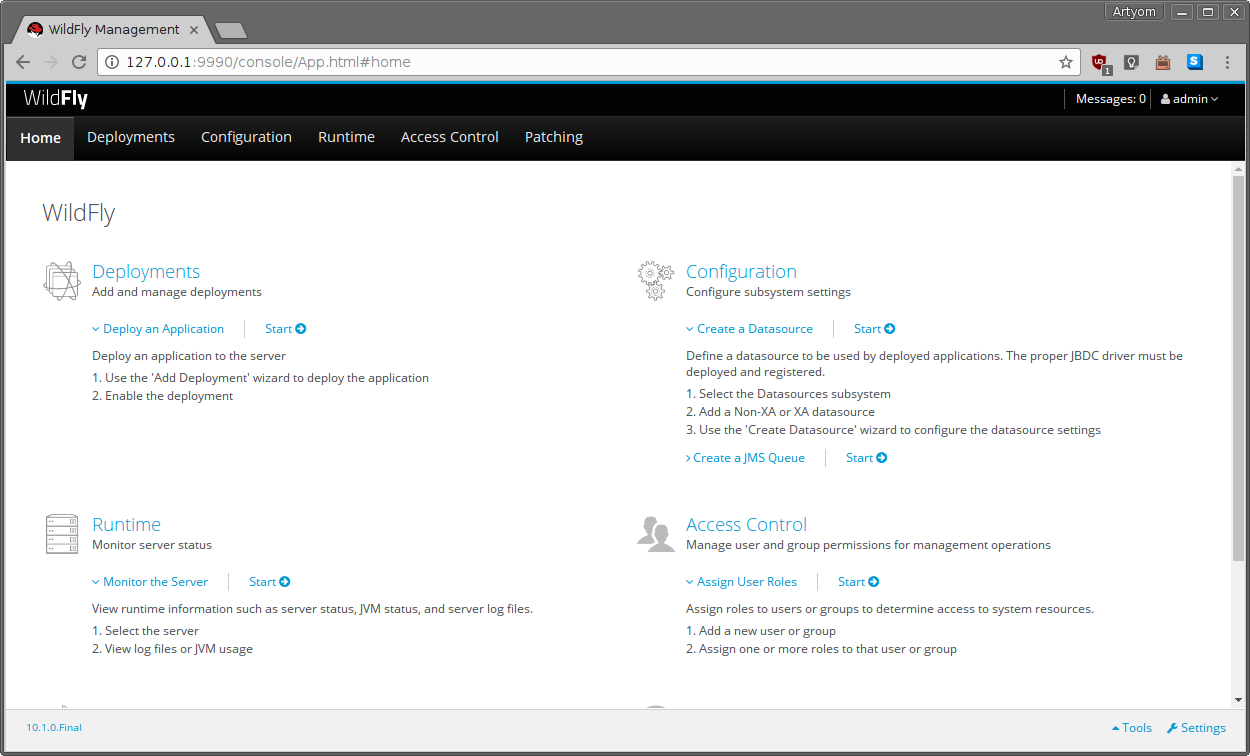
\includegraphics[width=\textwidth]{wildfly.png}
\caption{}
\end{figure}

В пункте Deployment выберем пункт Start:

\begin{figure}[H]
\centering
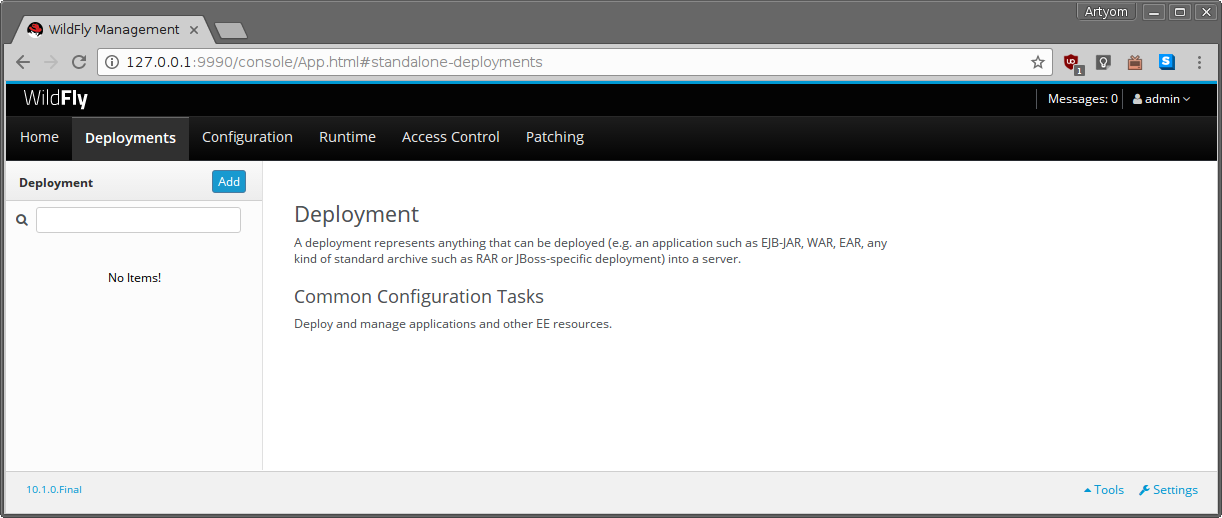
\includegraphics[width=\textwidth]{wildfly2.png}
\caption{}
\end{figure}

Далее необходимо нажать на кнопку Add. Откроется окно, где нужно выбрать собранный war-файл:

\begin{figure}[H]
\centering
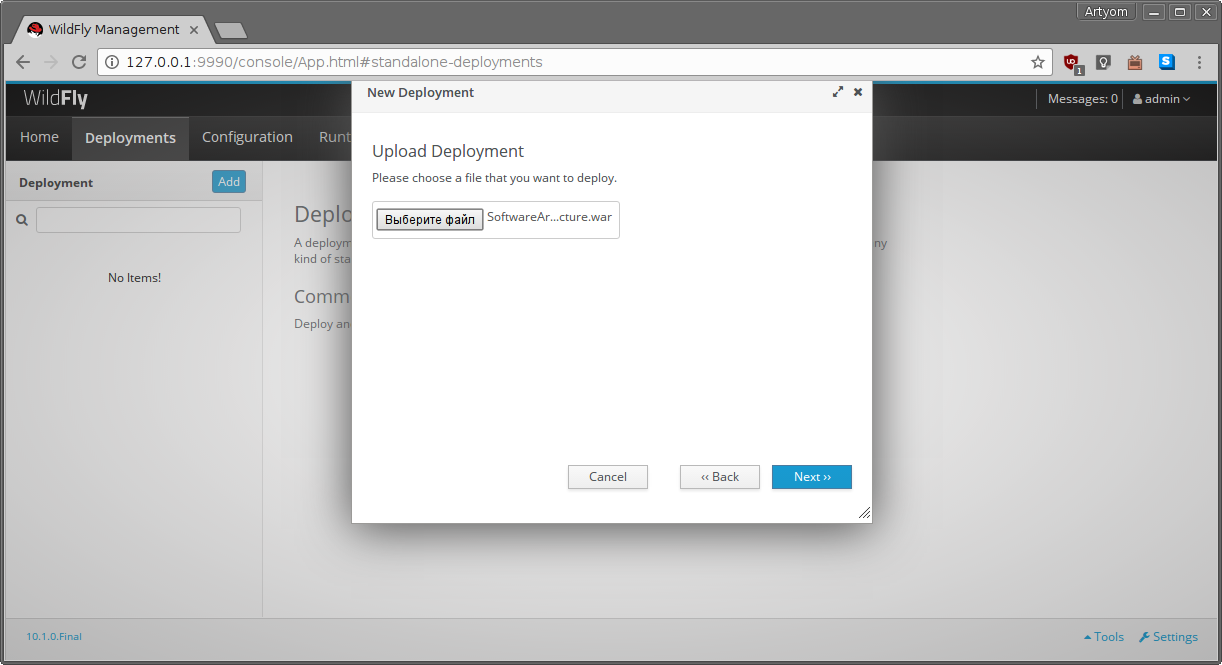
\includegraphics[width=\textwidth]{wildfly3.png}
\caption{}
\end{figure}

Развернутое приложение доступно по следующему адресу: \\ \url{http://127.0.0.1:8080/SoftwareArchitecture/}

\section{Выводы}
В рамках данного курса были изучены принципы разработки архитектуры программного обеспечения, а так же, следуя этим принципам, было разработано приложение.
в приложении было создано три слоя:

\begin{itemize}
\item
  Слой бизнес-логики
\item
  Слой хранения данных
\item
  Слой представления
\end{itemize}

Возможные пути улучшения разработанного приложения:

\begin{itemize}
\item Добавление возможности составления и верстки журнала. При этом возможно появление ещё одной роли - верстальщика. Результат верстки - электронный документ в одном из распространенных форматов (например, PDF).
\item Добавление интерфейса читателя
\end{itemize}